
\begin{frame}
  \maketitle
\end{frame}

\section{本編}
\begin{frame}{背景・目的}
  \begin{itemize}
  \item HPCにおけるネットワークをグラフで表現
    \begin{itemize}
    \item 無向(スイッチは双方向に通信可能)
    \item 正則(すべてのスイッチは同一個数のポートを有する)
    \item 平均頂点間距離が短いと遅延も短い
      \cite{Koibuchi2012,Singla2011}
    \item 平均頂点間距離が短い無向正則グラフを求める試み
      \cite{Fujita2015}
    \end{itemize}
  \end{itemize}
  \vspace{-1em}
  \begin{columns}[T]
    \begin{column}{.5\textwidth}
      \begin{itemize}
      \item \alert{一般化ムーアグラフ}
        \begin{itemize}
        \item 平均頂点間距離が理論的下界と等しい無向正則グラフ
          \cite{Cerf1973,Cerf1974Lower}
        \item 頂点数と次数の組によっては存在しない
        \item 一般化ムーアグラフを求める試み
          \cite{Yamamoto2016}
        \item 探索や存在判定のための効率的な方法は未知
        \end{itemize}
      \end{itemize}
    \end{column}
    \begin{column}{.5\textwidth}
      \begin{figure}
        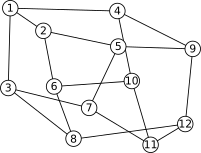
\includegraphics[width=.6\linewidth]{gmg-example}
        \caption{一般化ムーアグラフの例}
        \label{fig:gmg-example}
      \end{figure}
    \end{column}
  \end{columns}
  \begin{block}{}
    目的 : 一般化ムーアグラフの効率的探索法(存在判定法)の提案と評価
  \end{block}
\end{frame}

\begin{frame}[allowframebreaks]{探索アルゴリズム}
  \begin{theorem}
    \label{thm:gmg-geom}
    {\scriptsize
    正則グラフ$(n,k)$が一般化ムーアグラフであることの必要十分条件は
    次の二つの条件を同時に満たすことである.
    \begin{enumerate}
    \item 長さ$2Q$以下の閉路が存在しない.
      \label{itm:gmg-geom-1}
    \item $R=0$ならば直径が$Q$であり,$R>0$ならば直径が$Q+1$である.
      \label{itm:gmg-geom-2}
    \end{enumerate}
    \[ Q=\max\{q|n-1-\sum_{i=1}^{q}k(k-1)^{i-1}\geq 0\},\quad
    R=n-1-\sum_{i=1}^{Q}k(k-1)^{i-1} \]
    }
  \end{theorem}
  \vspace*{-1em}
  \begin{columns}
    \begin{column}{.4\textwidth}
      \begin{figure}
        \centering
        \includegraphics[height=.3\textheight]{feasible-edges-example-color}
        \caption{初期グラフと候補辺}
      \end{figure}
    \end{column}
    \begin{column}{.6\textwidth}
      \small
      \par 深さ優先探索に基づく
      \begin{enumerate}
      \item 初期グラフをスタックにプッシュする
      \item ポップしたグラフと,それに候補辺を追加したグラフを
        スタックにプッシュする
      \par 定理\ref{thm:gmg-geom}の条件に反するならプッシュしない
      \end{enumerate}
    \end{column}
  \end{columns}
\end{frame}

\begin{frame}{探索空間の削減}
  \begin{columns}[T]
    \begin{column}{.5\textwidth}
      \begin{itemize}
      \item 初期グラフの制限
      \end{itemize}
      \vspace*{-1em}
      \begin{figure}
        \centering
        \includegraphics[width=.7\columnwidth]
                        {initial-tree-cycle-example-color}
                        \caption{閉路を含むグラフ(閉路)}
      \end{figure}
      \vspace*{-2em}
      \begin{figure}
        \centering
        \includegraphics[width=.8\columnwidth]
                        {initial-spanning-tree-18-example-color}
                        \caption{全域木}
      \end{figure}
    \end{column}
    \begin{column}{.5\textwidth}
      \begin{itemize}
      \item 直径の下界を利用した枝刈り
      \item[] まだ見ていない候補辺をすべて追加したグラフの直径を計算
      \item[] 定理\ref{thm:gmg-geom}の条件\ref{itm:gmg-geom-2}に反するなら枝刈り
      \end{itemize}
      \begin{figure}
        \centering
        \includegraphics[width=.7\columnwidth]{max-graph-example-color}
        \caption{直径の下界の計算に用いるグラフ}
      \end{figure}
    \end{column}
  \end{columns}
\end{frame}

\begin{frame}{実験}
  \begin{itemize}
  \item 測定項目
    \begin{enumerate}
    \item 探索時間(10回の平均)
    \item 展開状態数(スタックからグラフを取り出した回数)
    \end{enumerate}
  \item パラメータ(頂点数$n$と次数$k$)
    \begin{itemize}
    \item[]\par$\begin{aligned}
      n &= 4,6,8,10,12,14,16,18 \\
      k &= 3
    \end{aligned}$
    \end{itemize}
    \vspace{1em}
    \par\begin{table}
    \scriptsize
    \caption{実行環境}
    \label{tab:env-lab}
    \centering
    \begin{tabular}{ll}
      \hline
      プロセッサ & Intel® Core™ i5-4670 CPU @ 3.40GHz × 4 \\ \hline
      メインメモリ & 5.8GiB \\ \hline
      ゲストOS & Ubuntu 16.04.3 LTS 64 ビット \\ \hline
      仮想化 & Oracle VirtualBox バージョン 5.1.18 \\ \hline
      ホストOS & Windows 8.1 64 ビット \\ \hline
      コンパイラ & gcc 5.4.0 \\ \hline
      グラフライブラリ & igraph 0.7.1-2.1 \\ \hline
      最適化フラグ & -Ofast \\ \hline
    \end{tabular}
    \end{table}
  \end{itemize}
\end{frame}

\begin{frame}{結果}
  \begin{columns}[T]
    \begin{column}{.5\textwidth}
      \begin{itemize}
      \item 全域木を使うと最速で最も展開状態数が少ない
      \item 閉路は頂点数12で基本より展開状態数が多い
        \begin{itemize}
        \item 候補辺が適切な順番でなく,正則グラフの判定が遅くなるため
        \end{itemize}
        \medskip
      \item 枝刈りによって展開状態数が減少する
      \item 小さい頂点数に対して探索時間が増加する
        \begin{itemize}
        \item 下記により効率化が無効になるため
        \end{itemize}
        \vspace*{-.5em}
        \begin{enumerate}
        \item 直径の計算が必要になること
        \item 多くのグラフの生成と破棄が発生すること
        \end{enumerate}
      \end{itemize}
    \end{column}
    \begin{column}{.5\textwidth}
      \centering
      \includegraphics[height=.35\textheight]{cmp-algo-time}
      \captionof{figure}{平均探索時間}
      \vfill
      \includegraphics[height=.35\textheight]{cmp-algo-state}
      \captionof{figure}{展開状態数}
    \end{column}
  \end{columns}
\end{frame}

\begin{frame}{まとめ}
  \begin{itemize}
  \item 一般化ムーアグラフの探索の探索空間の削減の効果を研究
    \begin{itemize}
    \item 全域木
    \item 直径の下界を利用した枝刈り
    \end{itemize}
  \item[] を使用することで効率良く探索できる
  \item 今後の課題
    \begin{itemize}
    \item 提案した初期グラフへの制限の妥当性の検証
    \item 一般化ムーアグラフが存在しないときの平均頂点間距離最小のグラフ
    \end{itemize}
  \end{itemize}
  \begin{figure}
    \centering
    \includegraphics[width=\textwidth]{gmg-existence-h}
    \caption{発見した一般化ムーアグラフの頂点数と次数の組}
  \end{figure}
\end{frame}

\appendix
\begin{frame}[allowframebreaks]{参考文献}
  \bibliography{../res/MyCollection}
\end{frame}

\begin{frame}[allowframebreaks]{一般化ムーアグラフの定義と例}
  \begin{definition}[Cerfら\cite{Cerf1973}]\rm\scriptsize
    \label{def:generalized-moore-graph}
    頂点数$n$,次数$k$の正則グラフ$G$を考える.
    $G$のすべての頂点$v$について,$v$との距離が$i$である頂点の数$c_i$が,
    \[\begin{aligned}
      c_i =
      \begin{cases}
        k(k-1)^{i-1}, & 1\leq i\leq Q(n,k) \\
        R(n,k), & i = Q(n,k)+1 \\
        0, & Q(n,k)+2\leq i \leq n-1
      \end{cases}
    \end{aligned}\]
    を満たすとき,$G$を\textbf{一般化ムーアグラフ}とよぶ.ただし,\\
    \[\begin{aligned}
      Q(n,k)&=\max\{q|n-1-\sum_{i=1}^{q}k(k-1)^{i-1}\geq 0\}\\
      R(n,k)&=n-1-\sum_{i=1}^{Q(n,k)}k(k-1)^{i-1}
    \end{aligned}\]
    である.
  \end{definition}
  \framebreak
  \begin{columns}[c]
    \begin{column}{.5\textwidth}
      \begin{itemize}
      \item 図\ref{fig:gmg-example}を例に考える
        \[ Q(12,3) = 2,\quad R(12,3) = 2 \]
      \item 頂点$1$に着目したとき距離が$i$の頂点数$c_i$は次の通り
        \begin{align*}
          c_1&= |\{2,3,4\}| = 3 = 3\cdot2^0 \\
          c_2&= |\{5,6,7,8,9,10\}| = 6 = 3\cdot2^1 \\
          c_3&= |\{11,12\}| = 2 = R(12,3) \\
          c_i&= 0\;(4\leq i\leq11)
        \end{align*}\par
      \end{itemize}
    \end{column}
    \begin{column}{.5\textwidth}
      \begin{figure}
        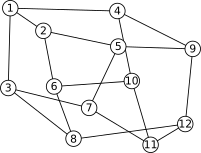
\includegraphics[width=.6\linewidth]{gmg-example}
        \caption*{
          {\usebeamercolor[fg]{caption name}図\ref{fig:gmg-example}}
          一般化ムーアグラフの例(再掲)
        }
      \end{figure}
    \end{column}
  \end{columns}
  \vspace{.5em}
  \begin{itemize}
  \item 他のすべての頂点について同じ距離と頂点数の関係を満たす
  \end{itemize}
\end{frame}

\begin{frame}{平均頂点間距離の下界}
  \begin{theorem}[Cerfら\cite{Cerf1974Lower}]\rm\scriptsize
    \label{thm:gmg-lower-bound}
    頂点数$n$,次数$k$の無向正則グラフの頂点間距離の総和の下界$S(n,k)$は
    \[
    S(n,k) = \sum_{(s,t)\in V\times V}d(s,t) =
    n \left[\ \sum^{Q}_{i=1}ik(k-1)^{i-1} + (Q+1)R\ \right]
    \]
    で与えられる.ただし,$Q$と$R$は定理\ref{thm:gmg-geom}に示した通り.
  \end{theorem}
  \par{\small 平均頂点間距離を求めるには$S(n,k)$を$n(n-1)$で割ればよい.}
  \begin{figure}
    \includegraphics[height=.3\textheight]{order-aspl}
    \caption{次数ごとの頂点数と平均頂点間距離の下界の関係}
  \end{figure}
  \vfill
\end{frame}

\begin{frame}{全域木の構築}
  \begin{enumerate}
  \item 頂点$1$と$2,\ldots,k+1$を隣接させる
    \begin{itemize}
    \item[] 頂点$2,\ldots,k+1$の集合を$L_1$とする
    \item[] 頂点$1$から距離が$i$である頂点の集合を$L_i$とする
    \end{itemize}
  \item $L_i$と$L_{i+1}$をつなげる
    \begin{itemize}
    \item $|L_{i+1}|=|L_i|(k-1)$
    \item $L_i=\{v,\ldots,v+|L_i|-1\},\,L_{i+1}=\{w,\ldots,w+|L_{i+1}|-1\}$
    \item[] (ただし$w=v+|L_i|$)として
    \item $j\in\{0,\ldots,|L_{i+1}|-1\}$に対して
      $w+j$と$v+(j\ \text{mod}\ |L_i|)$を隣接させる
    \end{itemize}
  \item 頂点数が$n$になるまで続ける
  \end{enumerate}

  \begin{figure}
    \centering
    \includegraphics<1|handout:0>[width=.4\textwidth]{spanning-tree-anim-1}
    \includegraphics<2|handout:0>[width=.4\textwidth]{spanning-tree-anim-2}
    \includegraphics<3|handout:0>[width=.4\textwidth]{spanning-tree-anim-3}
    \includegraphics<4|handout:0>[width=.4\textwidth]{spanning-tree-anim-4}
    \includegraphics<5|handout:0>[width=.4\textwidth]{spanning-tree-anim-5}
    \includegraphics<6|handout:0>[width=.4\textwidth]{spanning-tree-anim-6}
    \includegraphics<7|handout:0>[width=.4\textwidth]{spanning-tree-anim-7}
    \includegraphics<8|handout:0>[width=.4\textwidth]{spanning-tree-anim-8}
    \includegraphics<9|handout:0>[width=.4\textwidth]{spanning-tree-anim-9}
    \includegraphics<10|handout:0>[width=.4\textwidth]{spanning-tree-anim-10}
    \includegraphics<11|handout:0>[width=.4\textwidth]{spanning-tree-anim-11}
    \includegraphics<12|handout:0>[width=.4\textwidth]{spanning-tree-anim-12}
    \includegraphics<13|handout:0>[width=.4\textwidth]{spanning-tree-anim-13}
    \includegraphics<14|handout:0>[width=.4\textwidth]{spanning-tree-anim-14}
    \includegraphics<15>[width=.4\textwidth]{spanning-tree-anim}
    \caption{全域木初期グラフの構築}
  \end{figure}
\end{frame}

%\begin{frame}<handout:0>{付録}
%  ふろくです
%\end{frame}


